\let\cleardoublepage\clearpage
\chapter{Empirical Evaluation}
\label{chapter:Evaluation}

Main goal of this chapter is to assess how much is our IE checker
is efficient in terms of the count that it is able to detect true-positives,
false-negatives, false-positives, execution times and also its ability to fix
the detected bugs. Along with this, highlighting the research work that has
been carried out in this thesis. For the purpose of evaluation, we have used
the IE checker and the Juliet test cases CWE-524, CWE-534, CWE-535. All the results
from this evaluation will be represented in tables and also in graphs.



\section{Test Setup}

In order to fix the detected IE bugs, developed refactoring tool was used
for generating the two types of patches and then inserting in the
code program. Exisiting IE checker[ref] was used in order to detect the 
IE bugs in the code programs and also to classify the bug depending on the
bug description and its unique ID. Used 64-bit Linux Kernel 3.13.0-32.57, Intel i5-
3230 CPU @ 2.60GHz x 4 was used as a test system. Calculated the times needed to generated
all the patches and also the total time for detecting the bug. Measured
the times in milliseconds.


\section{Methodology}

The refactoring tool was run on 3 kinds of test programs with many flow variants
and generated two different types of code patches in order to 
automatically fix the bugs that were detected by the IE checker. Previously developed
IE checker and classification mechanism in order to differentiate different
types of bugs. Measured all the times required for running the checker,
for detecting the bug, for refactoring and also the overall overhead that occured
because of refactoring. Times were measured in milliseconds and then again
converted into seconds[s]. Program behaviour was preserved for all the program
inputs which did not trigger the bug. Some of the research questions that have been 
addressed are:
\begin{itemize}
 \item Overall computational overhead of the tool.
 \item Usefulness of the generated code patches.
 \item About the program behavior.
 \item Correctness
\end{itemize}

CWE- 526, CWE-534, CWE-535 were used as the test programs for running our already existing IE checker
because these test cases contain the bugs for which the IE checker was built.
All the test cases were also publicly online available in the 
Juliet test suite [ref]. The number of test programs present in CWE-526 are 18 Test Programs(TPr),
CWE-534 has 36 TPr and CWE-536 has 36 TPr. All these test programs CWE-526/534/535 were 
exported in to the eclipse workspace by already created Eclipse CDT project instance.

After all the test programs were imported into the Eclipse CDT workspace,
the existing IE checker which is an eclipse JDT plugin was made to 
run automatically for each test program available in the workspace.
This can be done by selecting the submenu "Run C/C++ Code analysis" after
right clicking on the selected test program. The following time were measured
and represented in the respective tables: time for running the checker for detecting the bug was
measured [ref], time for patch generation[], execution time for the test programs which belong
to the test case.
Also the number of true positives, false positives, true negatives and false negatives
were are also calculated and reperesented in the table~\ref{table:errors}. 
Following are the abbrevations in the table: True postives (TP), Lines of Code (LOC),
and these lines are excluding the code comments, False Positives (FP), False Negatives (FN),
Total True Positives (TTP). Developed tool was able to find 85 TPs out of 90 TPs
which are the available test programs. Tool was able to detect all the IE bugs.
But the programs containing the goto statements were not able to be tested since
the Codan API doesnot support building the Control Flow Graphs (CFGs) for the 
C source code containing goto statements. For example, goto A; .
Among all the test programs available in Juilet test suite CWE-526 has 1 program
which contians goto statement, 2 in CWE-534 and 2 in CWE-535. As a whole 5 programs
out of 90 test programs were able to be analyzed by building the CFGs. Therefore
,the overall test coverage reached to 94.44\%. It can be concluded that 
the tool would reach a test coverage of 100\% if this limitation was removed.


\begin{table}[h!]
\centering
 \begin{tabular}{||c |c |c |c |c| c|c||} 
 \hline
 \textbf{Test Programs} & \textbf{TP} & \textbf{LOC} & \textbf{FP} & \textbf{FN}& \textbf{TTP}&
 \textbf{TTP}\\ [0.5ex]
 \hline
CWE-526&18&960&0&0&17&18\\
\hline
CWE-534&36&5783&0&0&34&36\\
\hline
CWE-535&36&5273&0&0&34&36\\
\hline
Total&90&12016&0&0&85&90\\
\hline
 \hline
\end{tabular}
\caption{Measured values of CWE-526}
\label{table:errors}
\end{table}

It was already know the number of test programs that should have the bug marker icon in the
test program after running the IE checker using static analysis and 
also the count on how many should not have the bug marker icon ( 5 out of 90 test
programs will not contain the bug icon since it was not possible for running the
static analysis). Usually a bug icon is similar to the image of a bug and the description of the
bug is shown in the console view with a triangle symbol with an exclamation mark inside it.

We can see three different types of messages:
\begin{figure}[!htb]
\centering
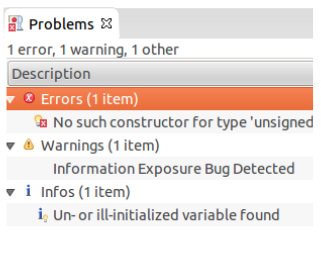
\includegraphics[width=0.5\textwidth]{png/Types.png}
\caption{Types of possible messages}
\label{fig:types}
\end{figure}\\

\begin{enumerate}
\item Errors
\item Warnings
\item Infos
\end{enumerate}

Errors are represented with red circle with a cross inside icon, Warnings are represented
with a traingle and exclamation mark inside icon, infos is represented with i symbol icon.
In this IE checker we do not use errors and infos but only the warnings
where the bug descripted will be displayed in the console view of
the Eclipse CDT instance after running the IE checker and detecting
the bugs as shown in figure~\ref{fig:types}. Therefore once the bugs are
detected and the bug mark icon is placed, one can see the traingle icon 
with exclamation mark inside in the console view. Once we click on the
message that has been generated by the Information exposure bug report
represented in figure~\ref{fig:types} then the cursor will be pointing
to the line number where the bug was found. There are different modes in which
the IE checker can be configured in order to launch the checker as shown 
in figure~\ref{fig:modes}. This bug triggering modes can be very useful during the 
software development by giving a chance to the developer on how to control
and when should eclipse trigger the bug detection analysis. This will help the
developer to avoid insertion of bugs during the software development.
\begin{figure}[!htb]
\centering
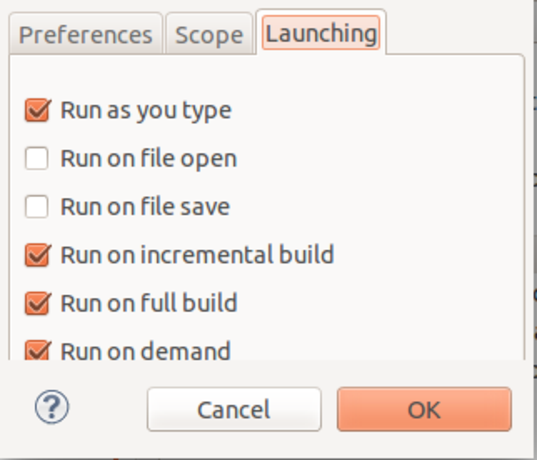
\includegraphics[width=0.4\textwidth]{pdf/modes.pdf}
\caption{Different running modes}
\label{fig:modes}
\end{figure}\\


\section{Results and Constraints}



\begin{table}[h!]
\centering
 \begin{tabular}{||c |c |c |c |c| c|c||} 
 \hline
 \textbf{Test Program} & \textbf{PGT[ms]} & \textbf{TT[ms]} & \textbf{No; of Paths} & \textbf{IP}& \textbf{Total no; of nodes}&
 \textbf{BDT[ms]}\\ [0.5ex] 
 \hline\hline
 CWE526-env-var-01 & 0.014 & 7.442 & 8 & 0& 250&7.428\\ 
 \hline
CWE526-env-var-02 & 0.02 & 4.082 & 12&0& 498&4.062\\ 
 \hline
 CWE526-env-var-03 & 0.013 & 3.603 & 12&0& 498&3.59\\ 
 \hline
 CWE526-env-var-04 & 0.017 & 3.306 & 12&0& 498&3.289\\ 
 \hline
 CWE526-env-var-05 & 0.017 & 3.456 & 12&0& 498&3.439\\ 
 \hline
 CWE526-env-var-06 & 0.01 & 3.455 & 12&0& 498&3.445\\ 
 \hline
 CWE526-env-var-07 & 0.011 & 3.386 & 12&0& 500&3.375\\ 
 \hline
 CWE526-env-var-08 & 0.01 & 3.169 & 12&0& 564&3.159\\ 
 \hline
 CWE526-env-var-09 & 0.008 & 3.241 & 12&0& 498&3.233\\ 
 \hline
 CWE526-env-var-10 & 0.012 & 3.373 & 12&0&498&3.361 \\ 
 \hline
 CWE526-env-var-11 & 0.014 & 3.207 & 12&0&564&3.193 \\ 
 \hline
 CWE526-env-var-12 & 0.017 & 3.116 &20&0& 1001&3.099\\ 
 \hline
 CWE526-env-var-13 & 0.013 & 3.236 & 12&0& 498&3.223\\ 
 \hline
 CWE526-env-var-14 & 0.014 & 3.239 & 12&0& 498&3.225\\ 
 \hline
 CWE526-env-var-15 & 0.014 & 3.272 & 12&0&507&3.258\\ 
 \hline
  CWE526-env-var-16 & 0.005 & 3.182 & 10&0& 356&3.177\\ 
 \hline
  CWE526-env-var-17 & 0.005 & 3.303 & 12&0& 533&3.298\\ 
 \hline
  CWE526-env-var-18 & 0 & 0 & 0&0& 0&0\\ 
 \hline
 \hline
\end{tabular}
\caption{Measured values of CWE-526}
\label{table:time1}
\end{table}

Table\ref{table:time1} depicts all the measured values for the test case 
CWE-526,Table\ref{table:time2} 
depicts all the measured values for the test case CWE-534 and
Table\ref{table:time3} depicts all the measured values for the test case CWE-535.The column
abbrevations are Path Generation Time (PGT), Total Time (TT), Influencible Paths (IP),
Bug Detection Time (BDT).

\begin{figure}[!htb]
\centering
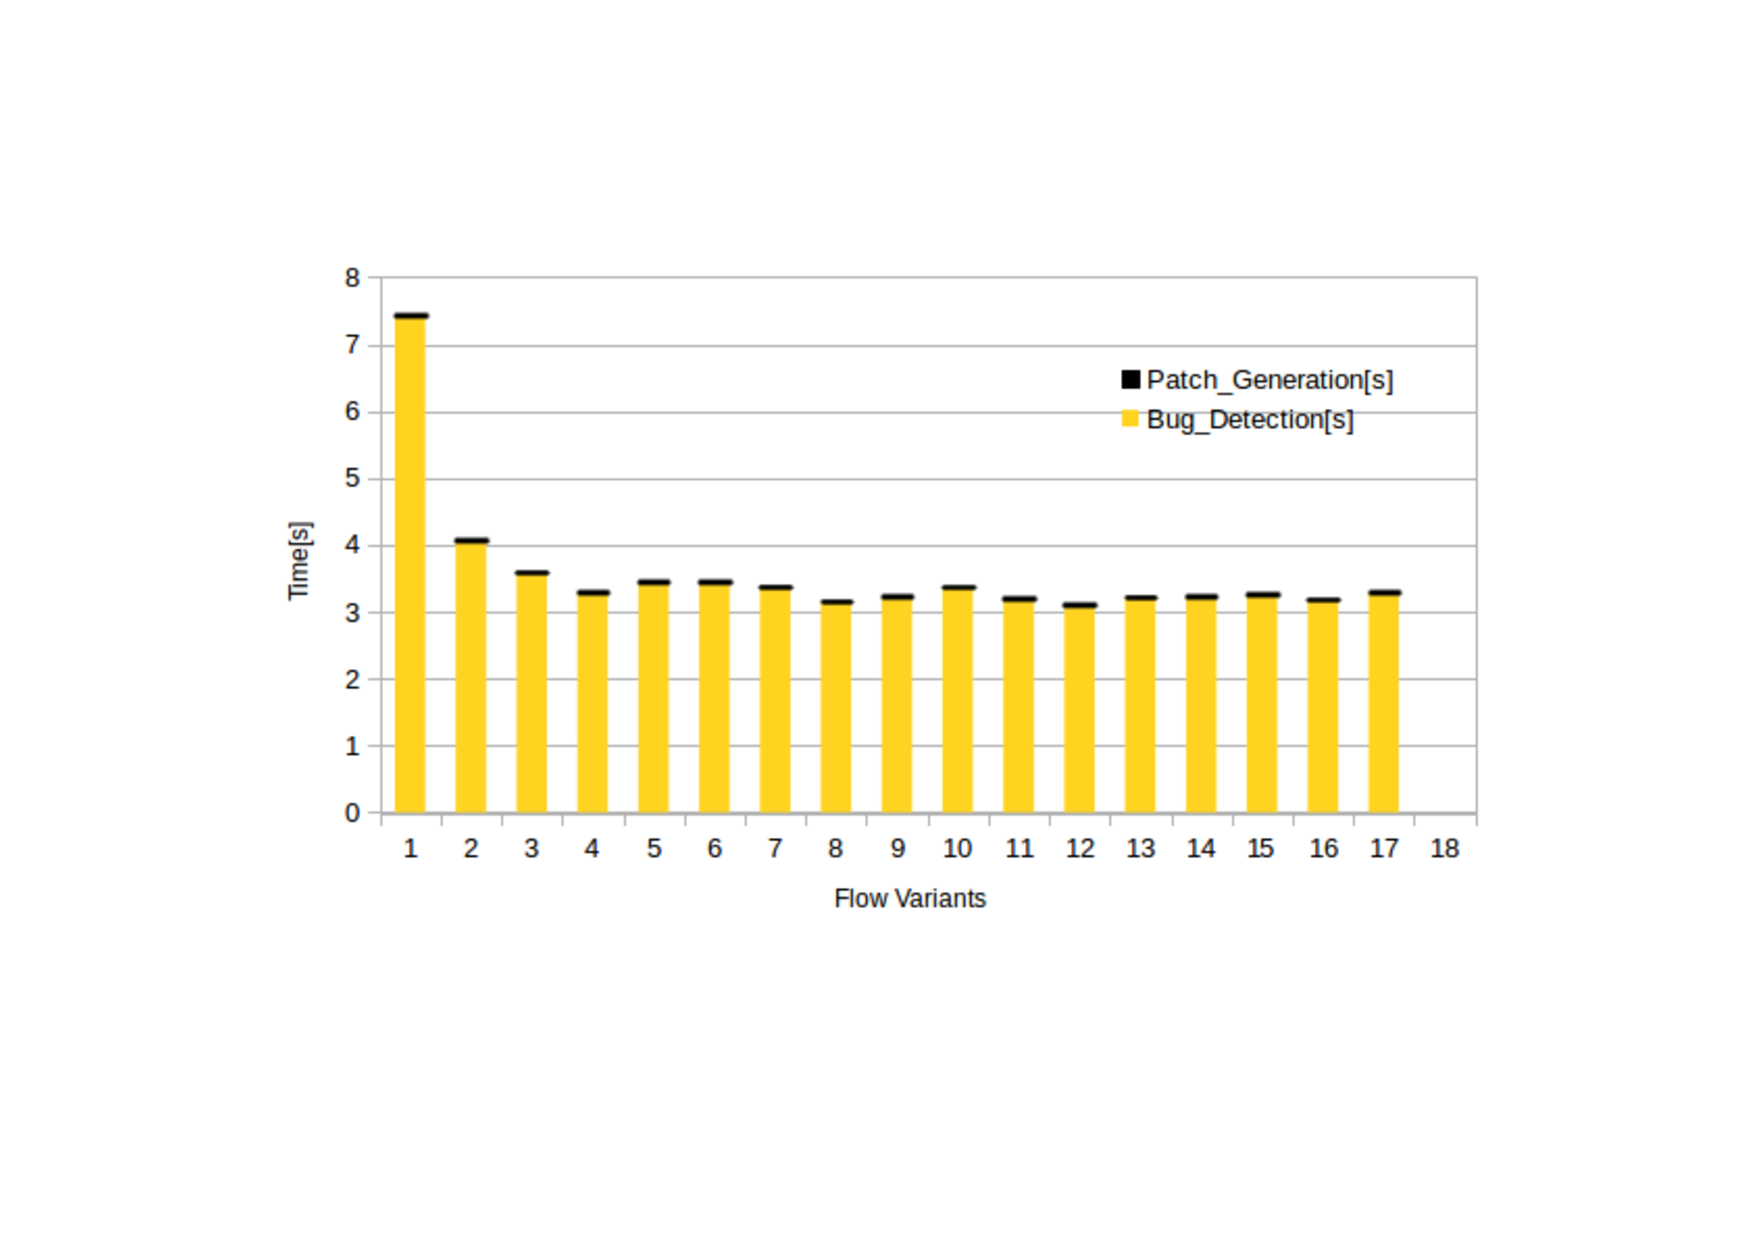
\includegraphics[trim=5.0cm 0.0cm 0.0cm 0.0cm, scale=0.7]{pdf/time1.pdf}
\vspace{-4.5cm}
\caption{Comparision between the patch generation and bug detection times of CWE-526}
\label{fig:time1}
\end{figure}


\begin{table}[h!]
\centering
 \begin{tabular}{||c |c |c |c |c| c|c||} 
 \hline
 \textbf{Test Program} & \textbf{RT} & \textbf{TT} & \textbf{No; of Paths} & \textbf{IP}& \textbf{Total no; of nodes}& \textbf{BDT[ms]} \\ [0.5ex] 
 \hline\hline
 CWE534-debug-char-01 & 0.004 & 5.644 & 87 & 0& 7560&5.64 \\ 
 \hline
CWE534-debug-char-02 & 0.043 &  9.688 & 372&0& 48645&9.645 \\ 
 \hline
 CWE534-debug-char-03 & 0.01& 8.649 & 372&0& 48645&8.639 \\ 
 \hline
 CWE534-debug-char-04 & 0.013 & 8.62 & 370&0& 48552&8.607 \\ 
 \hline
 CWE534-debug-char-05 & 0.016 & 8.487 & 372&0& 48645&8.471 \\ 
 \hline
 CWE534-debug-char-06 & 0.015 & 8.264& 371&0& 48609&8.249 \\ 
 \hline
 CWE534-debug-char-07 & 0.014 & 8.352 & 372&0& 48645&8.338 \\ 
 \hline
 CWE534-debug-char-08 & 0.018 &6.421 & 198&0& 30141&6.403 \\ 
 \hline
 CWE534-debug-char-09 & 0.051 &10.177 &372&0& 48645&10.126 \\ 
 \hline
 CWE534-debug-char-10 & 0.022 & 7.894& 278&0&36495&7.872  \\ 
 \hline
 CWE534-debug-char-11 & 0.017 &8.891& 372&0&51699&8.874  \\ 
 \hline
 CWE534-debug-char-12 & 0.007 & 7.363 &308&0& 32341&7.356 \\ 
 \hline
 CWE534-debug-char-13 & 0.015 &48.654 & 372&0& 48645&48.63 \\ 
 \hline
 CWE534-debug-char-14 & 0.02 & 8.517 & 372&0& 48645&8.497 \\ 
 \hline
 CWE534-debug-char-15 & 0.011 & 8.555 & 372&0&49014&8.544 \\ 
 \hline
  CWE534-debug-char-16 & 0.003 &4.266 & 92&0& 8551&4.263 \\ 
 \hline
  CWE534-debug-char-17 & 0.002 & 3.989 & 57&0& 5905&3.987 \\ 
 \hline
  CWE534-debug-char-18 & 0 & 0 & 0&0& 0&0 \\ 
  \hline
  CWE534-debug-wchar-01 & 0.003 &3.846 &61 & 0& 5816& 3.843\\ 
 \hline
CWE534-debug-wchar-02 & 0.005 & 5.726 & 204&0& 29470& 5.721\\ 
 \hline
 CWE534-debug-wchar-03 & 0.005 &5.662 & 204&0& 29470& 5.657\\ 
 \hline
 CWE534-debug-wchar-04 & 0.019 & 5.73 & 204&0& 29470&5.711 \\ 
 \hline
 CWE534-debug-wchar-05 & 0.004 & 5.806 & 204&0& 29470& 5.802\\ 
 \hline
 CWE534-debug-wchar-06 & 0.005 & 5.711 & 204&0& 29470& 5.706\\ 
 \hline
 CWE534-debug-wchar-07 & 0.006 & 5.666 & 204&0& 29470&5.66 \\ 
 \hline
 CWE534-debug-wchar-08 & 0.008 & 5.619 & 204&0& 31084&5.611 \\ 
 \hline
 CWE534-debug-wchar-09 & 0.007 & 5.674 & 204&0& 29470& 5.667\\ 
 \hline
 CWE534-debug-wchar-10 & 0.003 & 5.732 & 202&0&29276&5.729  \\ 
 \hline
 CWE534-debug-wchar-11 & 0.005 & 5.718 &204&0&31084& 5.713 \\ 
 \hline
 CWE534-debug-wchar-12 & 0.003 &6.337 &211&0& 24400& 6.334\\ 
 \hline
 CWE534-debug-wchar-13 & 0.004 & 5.903 & 203&0& 29404&5.899 \\ 
 \hline
 CWE534-debug-wchar-14 & 0.005 & 5.548 & 204&0& 29470&5.543 \\ 
 \hline
 CWE534-debug-wchar-15 & 0.003 & 5.779 & 199&0&29323&5.776 \\ 
 \hline
  CWE534-debug-wchar-16 & 0.001 & 3.847 & 66&0& 6608&3.846 \\ 
 \hline
  CWE534-debug-wchar-17 & 0.002 & 4.027 & 78&0& 8752&4.025 \\ 
 \hline
  CWE534-debug-wchar-18 & 0 & 0 & 0&0& 0& 0\\
 \hline
 \hline
\end{tabular}
\caption{Measured values of CWE-534}
\label{table:time2}
\end{table}

\begin{figure}[!htb]
\centering
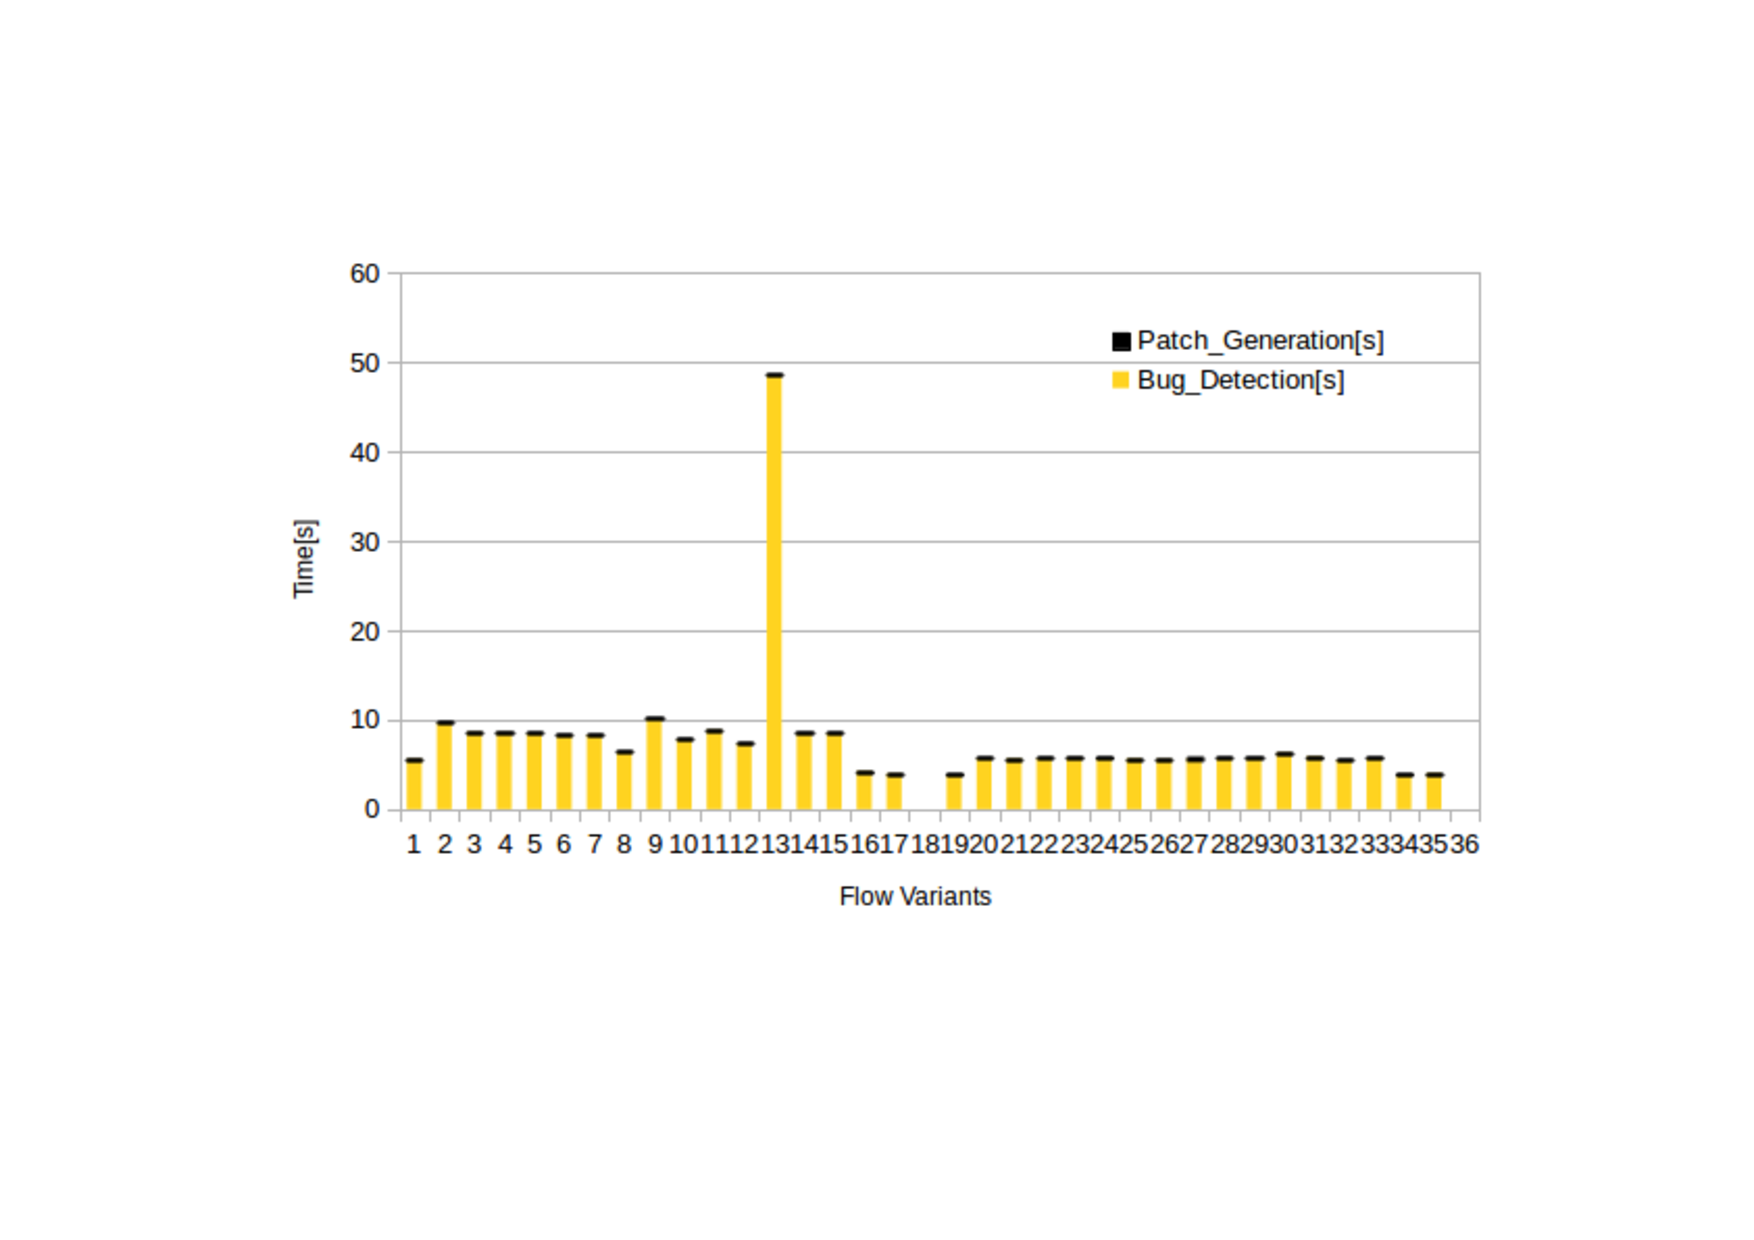
\includegraphics[trim=5.0cm 0.0cm 0.0cm 0.0cm, scale=0.7]{pdf/time2.pdf}
\vspace{-4.5cm}
\caption{Comparision between the patch generation and bug detection times of CWE-534}
\label{fig:time2}
\end{figure}
\begin{table}[h!]
\centering
 \begin{tabular}{||c |c |c |c |c| c|c||} 
 \hline
 \textbf{Test Program} & \textbf{RT} & \textbf{TT} & \textbf{No; of Paths} & \textbf{IP}& \textbf{Total no; of nodes}&\textbf{BDT[ms]}\\ [0.5ex] 
 \hline\hline
 CWE535-shell-char-01 & 0.001 & 3.946 &67 & 0&5239& 3.945\\ 
 \hline
CWE535-shell-char-02 & 0.014 & 7.316 & 288&0& 33700& 7.302 \\
 \hline
 CWE535-shell-char-03 & 0.013 & 7.379 & 288&0& 33700&7.366 \\ 
 \hline
 CWE535-shell-char-04 & 0.015 & 7.472 & 288&0& 33700&7.457 \\ 
 \hline
 CWE535-shell-char-05 & 0.025 & 7.336 & 288&0& 33700& 7.311\\ 
 \hline
 CWE535-shell-char-06 & 0.014 & 7.41 & 288&0& 33700&7.396 \\ 
 \hline
 CWE535-shell-char-07 & 0.017 & 7.257 & 288&0& 33700&7.24 \\ 
 \hline
 CWE535-shell-char-08 & 0.014 & 7.392 & 288&0& 36070&7.378 \\ 
 \hline
 CWE535-shell-char-09 & 0.018 & 7.367 & 288&0& 33700&7.349 \\ 
 \hline
 CWE535-shell-char-10 & 0.005 & 4.797 & 112&0&12794 &4.792 \\ 
 \hline
 CWE535-shell-char-11 & 0.019 & 7.25 & 288&0&36070& 7.231 \\ 
 \hline
 CWE535-shell-char-12 &0.007  & 6.509 &236&0& 22707& 6.502\\ 
 \hline
 CWE535-shell-char-13 &0.012  & 7.285 & 288&0& 33700&7.273 \\ 
 \hline
 CWE535-shell-char-14 & 0.018 & 7.547 & 288&0& 33700& 7.529\\ 
 \hline
 CWE535-shell-char-15 & 0.015 & 6.921 &254&0&29867&6.906 \\ 
 \hline
  CWE535-shell-char-16 & 0.004 & 4.223 & 71&0& 6007& 4.219\\ 
 \hline
  CWE535-shell-char-17 & 0.003 &4.491 & 92&0& 8910&4.488 \\ 
 \hline
  CWE535-shell-char-18 & 0 & 0 & 0&0& 0&0 \\ 
  \hline
  CWE535-shell-wchar-01 & 0.001 & 3.645 &48 & 0& 4198&3.644 \\ 
 \hline
CWE535-shell-wchar-02 & 0.005 & 5.223 & 165&0& 21568&5.218 \\ 
 \hline
 CWE535-shell-wchar-03 & 0.006 & 5.208 & 165&0& 21568& 5.202\\ 
 \hline
 CWE535-shell-wchar-04 & 0.005 & 5.28 & 165&0& 21568& 5.275\\ 
 \hline
 CWE535-shell-wchar-05 & 0.005 &5.248 & 165&0& 21568& 5.243\\ 
 \hline
 CWE535-shell-wchar-06 & 0.008 & 5.47 & 165&0& 21568&5.462 \\ 
 \hline
 CWE535-shell-wchar-07 & 0.006& 5.216 & 165&0& 21568&5.21 \\ 
 \hline
 CWE535-shell-wchar-08 & 0.007 & 5.543 & 165&0& 22876&5.536 \\ 
 \hline
 CWE535-shell-wchar-09 & 0.005 & 5.24 & 165&0& 21568&5.235 \\ 
 \hline
 CWE535-shell-wchar-10 & 0.008 & 5.036 & 165&0&21568 & 5.028\\ 
 \hline
 CWE535-shell-wchar-11 & 0.007 & 5.326 & 165&0&22876 &5.319 \\ 
 \hline
 CWE535-shell-wchar-12 & 0.004 & 5.245 &170&0& 18037&5.241 \\ 
 \hline
 CWE535-shell-wchar-13 & 0.01 &5.218 & 165&0& 21568&5.208 \\ 
 \hline
 CWE535-shell-wchar-14 & 0.006 & 5.521 &170&0& 21568&5.515 \\ 
 \hline
 CWE535-shell-wchar-15 & 0.005 & 5.401 & 165&0&21730&5.396 \\ 
 \hline
  CWE535-shell-wchar-16 & 0.001 & 3.914 & 165&0& 4922& 3.913\\ 
 \hline
  CWE535-shell-wchar-17 & 0.006 & 5.561 & 165&0& 21568&5.555 \\ 
 \hline
  CWE535-shell-wchar-18 & 0 & 0 & 0&0& 0& 0\\
 \hline
 \hline
\end{tabular}
\caption{Measured values of CWE-535}
\label{table:time3}
\end{table}

\begin{figure}[!htb]
\centering
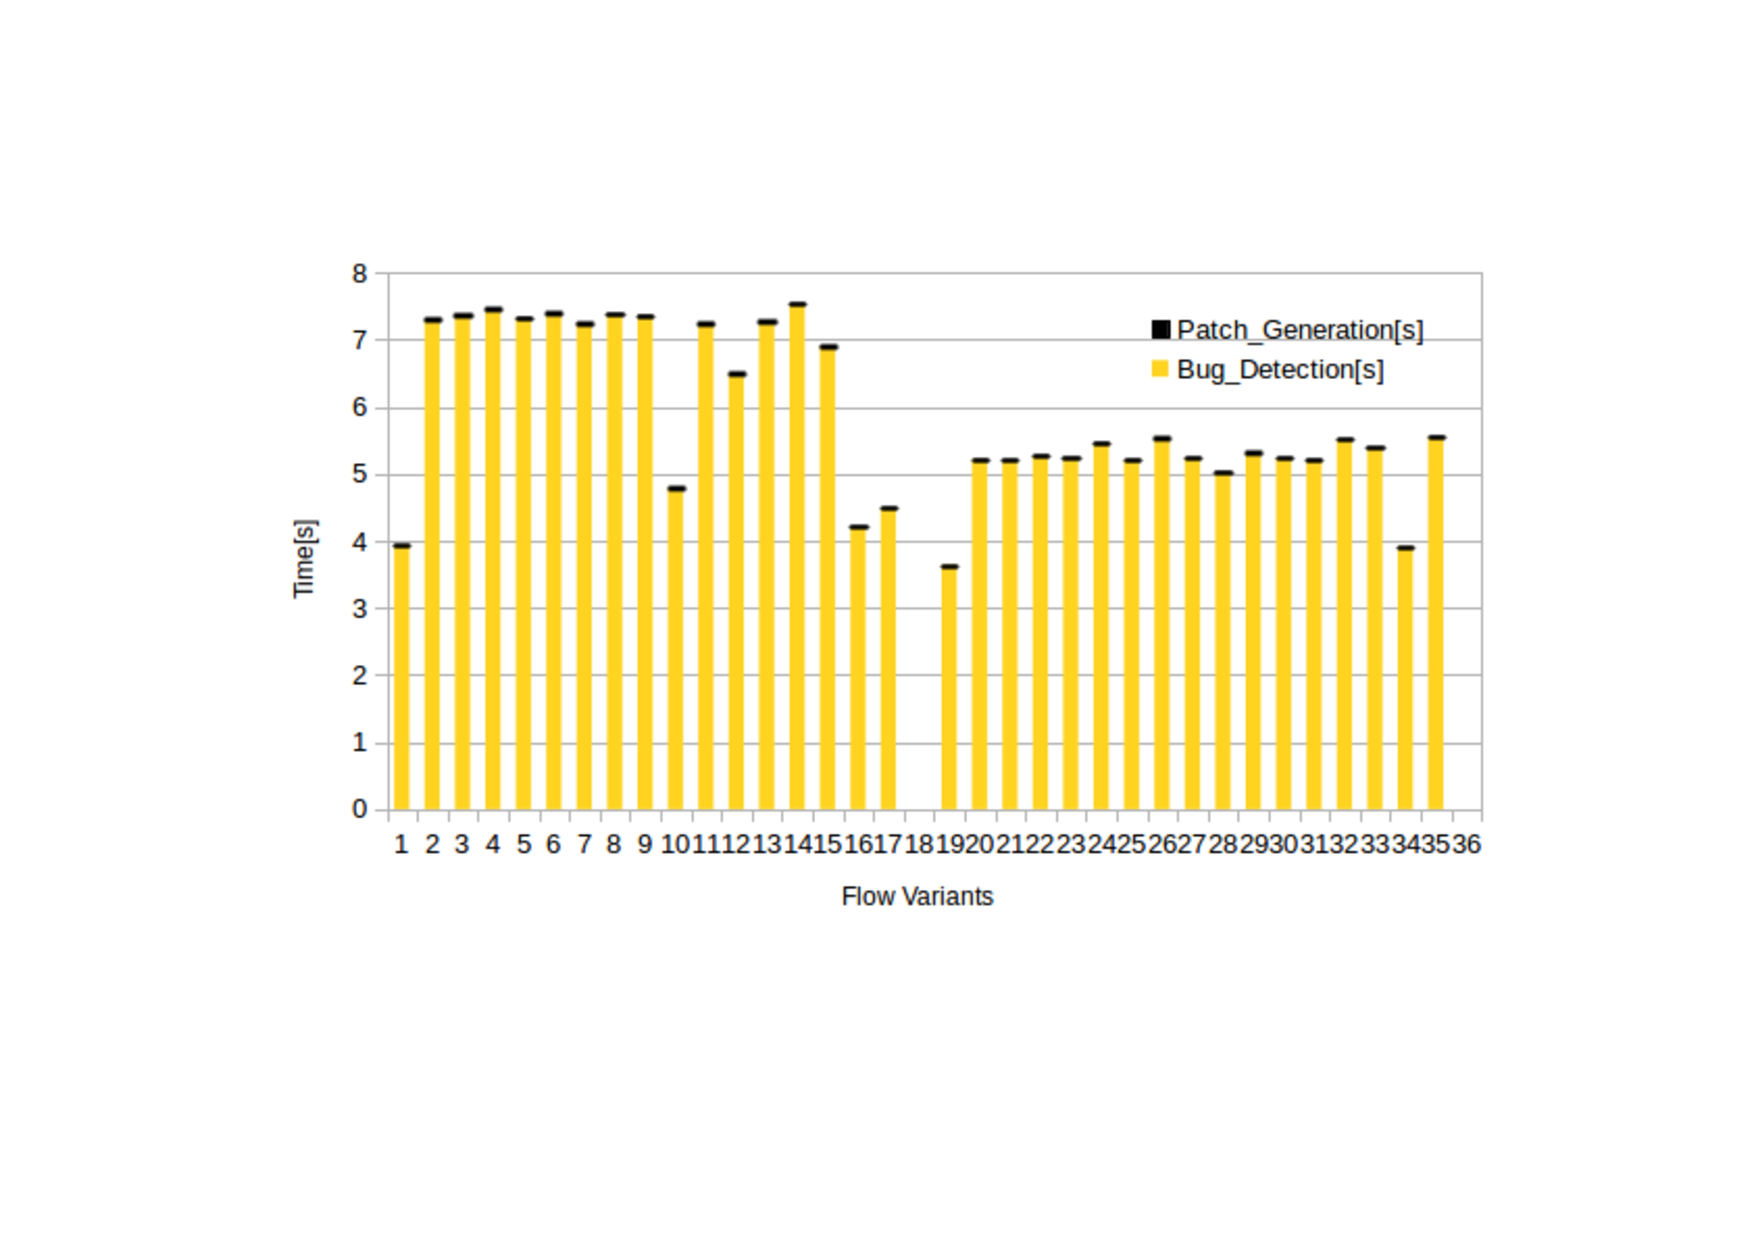
\includegraphics[trim=5.0cm 0.0cm 0.0cm 0.0cm, scale=0.7]{pdf/time3.pdf}
\vspace{-4.5cm}
\caption{Comparision between the patch generation and bug detection times of CWE-535}
\label{fig:time3}
\end{figure}
\section{Efficiency and Overhead}
Figure~\ref{fig:time1} shows the results when 18 C/C++ programs
of the test case CWE-526 from juilet test suite were run. The black bars above
the yellow bars indicate the overhead introduced due to the patch generation
and the yellow bars indicate the time taken for the bug detection. The total
overhead introduced for running these 18 test programs is 0.35\% which was
obtained by comparing the patch generation time (0.214[s]) with the bug detection
time (60.854[s]) 61.068[s]-0.214[s] which can be observed from the table
~\ref{table:overall}.


Figure~\ref{fig:time2} shows the results when 34 C/C++ programs
of the test case CWE-534 from juilet test suite were run out
of 36 test cases because the SMT solver used
could build the CFG for the test cases containing goto statements. The black bars above
the yellow bars indicate the overhead introduced due to the patch generation
and the yellow bars indicate the time taken for the bug detection. The total
overhead introduced for running these 34 test programs is 0.13\% which was
obtained by comparing the patch generation time (0.369[s]) with the bug detection
time (264.384[s]) 264.753[s]-0.369[s] which can be observed from the table
~\ref{table:overall}



Figure~\ref{fig:time3} shows the results when 34 C/C++ programs
of the test case CWE-535 from juilet test suite were run out
of 36 test cases because the SMT solver used
could build the CFG for the test cases containing goto statements. The black bars above
the yellow bars indicate the overhead introduced due to the patch generation
and the yellow bars indicate the time taken for the bug detection. The total
overhead introduced for running these 34 test programs is 0.15\% which was
obtained by comparing the patch generation time (0.309[s]) with the bug detection
time (198.884[s]) 199.193[s]-0.309[s] which can be observed from the table
~\ref{table:overall}

\begin{table}[h!]
\centering
 \begin{tabular}{||c |c |c |c ||} 
 \hline
 \textbf{Test Programs} & \textbf{TPGT} & \textbf{OTT} & \textbf{TBDT[ms]}\\ [0.5ex] 
 \hline\hline
 CWE-526&0.214&61.068&60.854\\
 \hline
 CWE-534&0.369&264.753&264.384\\
 \hline
 CWE-535&0.309&199.193&198.884\\
 \hline
Total&0.892&525.014&524.122\\
 \hline\hline
\end{tabular}
\caption{Overall Overhead}
\label{table:overall}
\end{table}

\begin{figure}[!htb]
\centering
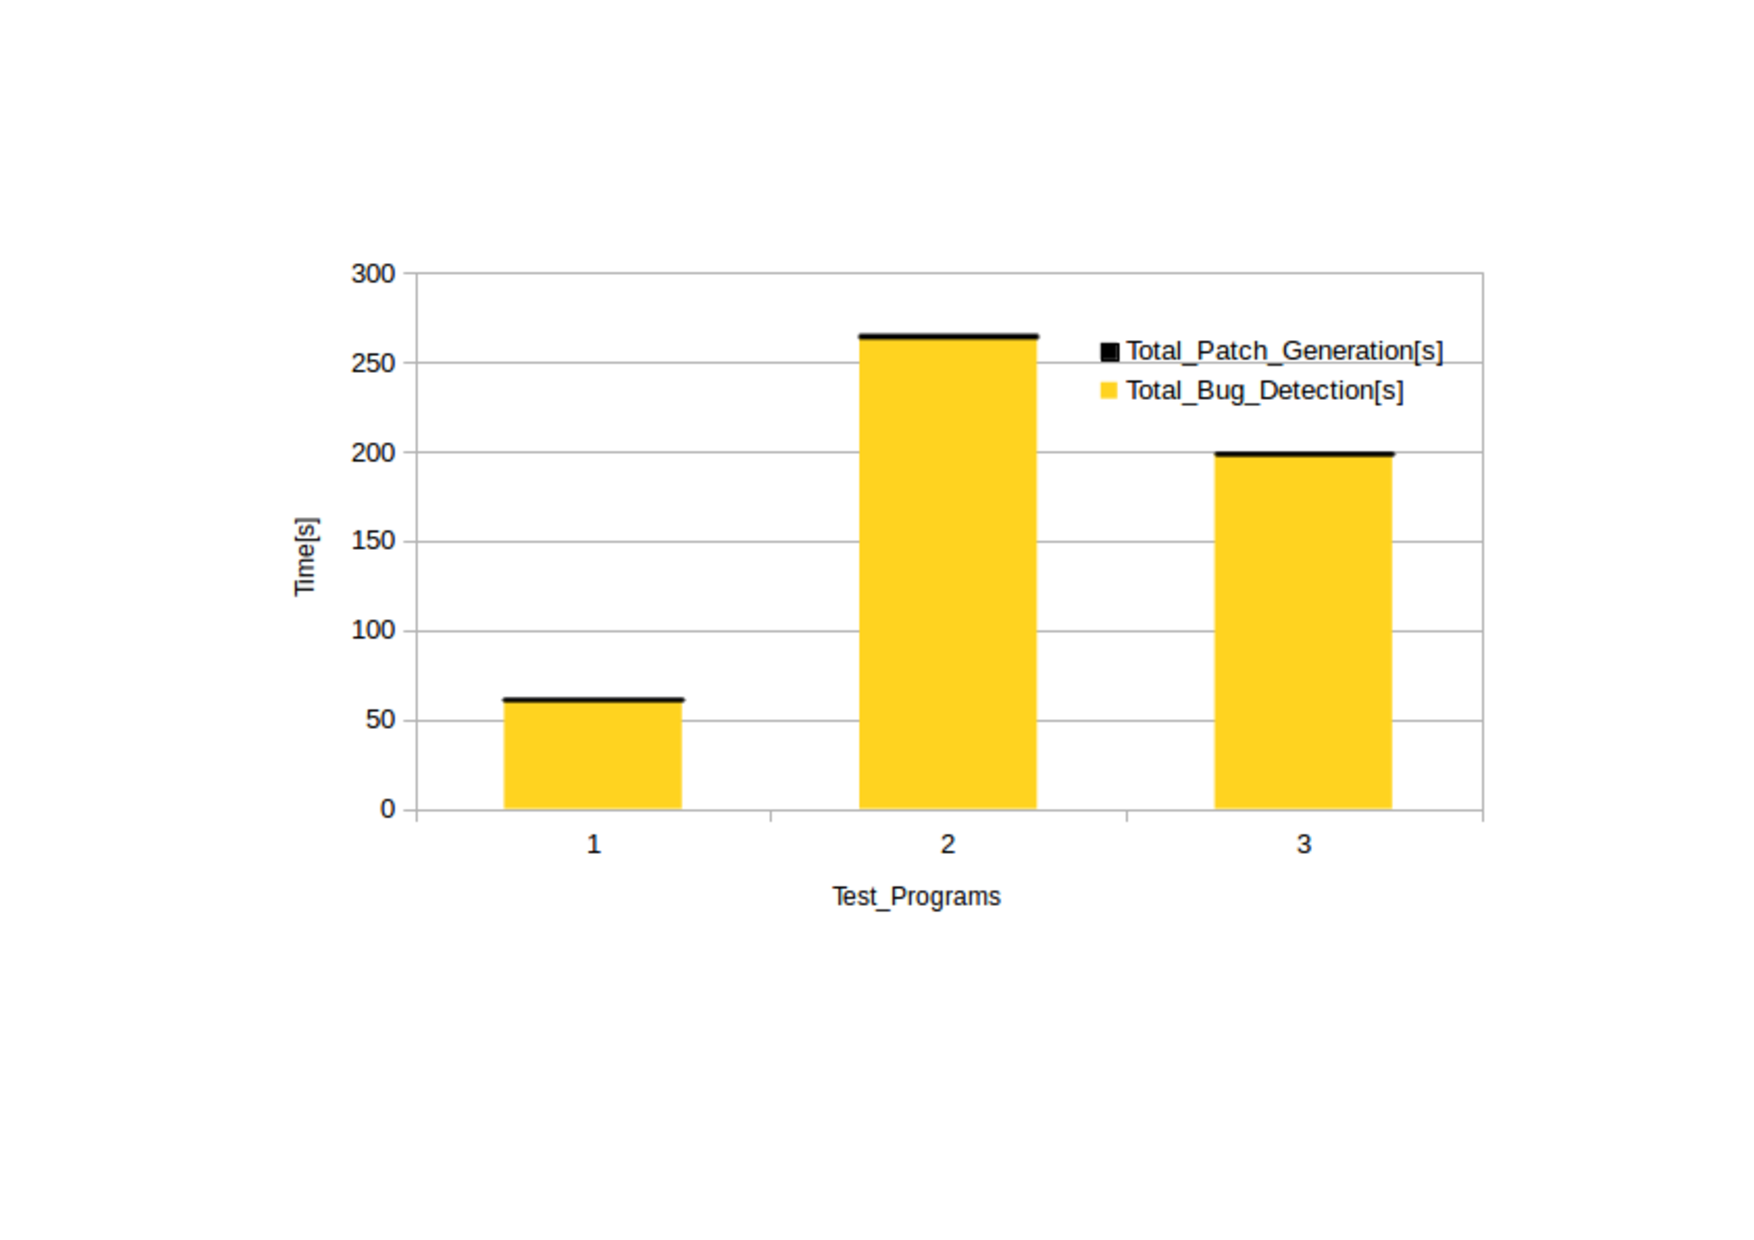
\includegraphics[trim=5.0cm 0.0cm 0.0cm 0.0cm, scale=0.75]{pdf/overall.pdf}
\vspace{-4.5cm}
\caption{Overall overhead}
\label{fig:overall}
\end{figure}
\section{Program Behaviour}
Program behaviour tells us if the newly inserted code patch changes the
behaviour of the program or not. Here program behaviour means
that the inserted code patches should not be able to influence the
already existing program paths. The abbrevation form the 
table~\ref{table:behavior}
IPa(Influencible paths), IP(Influencible Programs), \% Ratio represents
the ratio between the total number of programs to the total number of
influencible programs which contains atleast one influencible path.
Based on the decision made at the time for running the localizer,
which means there exits a not-in-place fix also. So after finding the 
not-in-place fix and inserting the code patch into the program form
refactoring then the program paths are then verified in order 
to check if the inserted code patch would change the program behaviour
or not. 


After verifying for the influencible paths, if it finds any such
influencible paths then the refactorings are not at all generated and
the decision is left to the programmer to refactor the code 
or not. This way the change of program behaviour can be avoided by not
proposing the refactorings at all. Change in program behavior after the 
patch insertion was completely avoided since the buggy variables found in the
test programs are all independent variables. So, if any dependant variables are
found later in the test programs then the choice of patch insertion is left to the 
user. From table~\ref{table:behavior}, one can observe the column 3 tells us
that there were no programs with influencible paths and column 4 tells us
that there were no infulencible paths at all.
Some of the test cases in the test programs CWE-526, CWE-534 and CWE-535 like
CWE526-Env-Var-18, CWE534-Debug-Log-char-18
, CWE534-Debug-Log-wchar-t-18, CWE535-Shell-Error-char-18
, CWE535-Shell-wchar-t-18 , a total of 5 programs
couldnot be verified. These programs contain the goto statements for which the 
SMT solver couldnot generate the executable paths and as a results no program
patches were generated. Thus, it can be concluded that
the program behavior is not changed at all.

\begin{table}[h!]
\centering
 \begin{tabular}{||c |c |c |c |c||} 
 \hline
\textbf{Test Programs} & \textbf{TTP} & \textbf{IP} & \textbf{IPa} & \textbf{\% Ratio}\\ [0.5ex] 
 \hline\hline
 CWE-526&18 &0 & 0& 0\\
 \hline
 CWE-534&36 &0 &0 &0 \\
 \hline
 CWE-535&36 &0 & 0 & 0\\
 \hline
 Total&90&0&0&0\\
  \hline\hline
\end{tabular}
\caption{Results of bug fixing}
\label{table:behavior}
\end{table}


\section{Usefulness of the generated Patches}
The usefulness of the generated patches is addressed by the following scenarios:
First scenario is by verifying if the generated code patches are syntactically
correct or not and also if the refactored code after the patch insertion can be
recompiled. Second, verifying if the inserted code patch was useful in removing
the detected bugs or not. Table~\ref{table:fixes} column 4 shows the usefulness
of the "not-in-place-fix", column 1 of table~\ref{table:fixes} shows 
the name of the test programs, column 3 of table~\ref{table:fixes} shows
the usefulness of the "in-place-fix". The results of the recompilation after
patch insertions of "in-place-fix" and "not-in-place-fix" is shown in the
column 2 of table~\ref{table:fixes}. As a result column 3 and column 4 of table
~\ref{table:fixes} tells us that the "in-place-fix" and the  "not-in-place-fix"
were useful in removing the detected bugs.


Here, in the test programs CWE-526, CWE-534, CWE-535 we can observe that there
are no influencible paths since there are not dependent variables in the 
detected bugs which can influence other variables further on in the program. 
Some of the test cases in the test programs CWE-526, CWE-534 and CWE-535 like
CWE526-Env-Var-18, CWE534-Debug-Log-char-18
, CWE534-Debug-Log-wchar-t-18, CWE535-Shell-Error-char-18
, CWE535-Shell-wchar-t-18 , a total of 5 programs
couldnot be verified. These programs contain the goto statements for which the 
SMT solver couldnot generate the executable paths and as a results no program
patches were generated. Therefore, it can be concluded that the program 
behavior will not be changed due to the insertion of this code patches
in order to fix the bugs.



\begin{table}[h!]
\centering
 \begin{tabular}{||c |c |c |c ||} 
 \hline
\textbf{Test Programs} & \textbf{Recompile} & \textbf{in-place-fix} & \textbf{not-in-place-fix}\\ [0.5ex] 
 \hline\hline
 CWE-526& \checkmark&\checkmark&\checkmark \\
 \hline
 CWE-534&\checkmark& &\checkmark \\
 \hline
 CWE-535& \checkmark& &\checkmark \\
  \hline\hline
\end{tabular}
\caption{Results of bug fixing}
\label{table:fixes}
\end{table}
\section{Threats to Validity}
\subsection{External Validity:}
In external validity we deal with the ability to generalize the empirically
evaluated results. In the empirical evaluation that had been carried out 3
test cases, a total of 90 test programs were used. But there are even more
other factors related to the testing platform and also the evaluation which 
could impact the results obtained.

In general the developed IE checker and the bug fixing can be used to other
test cases also. If other test cases doesnot contain any function models
in SAE then, First all the function models have to be defined, second all
the variables which are confidential have to be tainted. Later on the IE checker
has to be run and then based on the bug report the refactoring patch has to be decided.
Once the patch is generated, it then has to inserted in order to get the refactored
bug free code. The patch generation approach is also generalized which includes
the steps like detecting the failure, diagnosing the bug, localizing the bug cause,
and the repair inference). The overall overhead that has been acquired
is 0.17\% which is negligble when compared with the execution time.

Presently the available function models are less but in order to defined new
function models, one has to follow the same design pattern. Every
function model has a number of 5 methods. And all the code used for defining
a function model is almost the same for other function models,so one can reuse the 
same code. This leads to high level of resuse of code.

\subsection{Internal Validity:}
Internal validity deals with the ability to draw some conclusions about
the experimental conditions which could make any difference if something is
altered in those conditions because the experimental conditions could be either
dependent or independent experimental conditions. The definitions of sink and source
may sometimes lead to errors or biased for the test programs contianing many lines
of code. For the test cases used in thesis are not error prone.

All the test programs which we have used are all publicly available in the
Juliet test suite. The test programs were not at all modified. If the execution
times which have been calculated are not accurate then the calculated overhead
may mislead. The decisions made for the patch generation and selection of
patch according to the bug are static. Therefore this will not lead to any overhead
introduced by the developed tool. If the IE checker fails to detect the type of the
bug then the approach may not work at all or can also suffer from imprecision.

Therefore all these constraints does not pose any internal, external threats
to validity.


\chapter{Conclusion and Future Work}
\label{chapter:Conclusion}

It has been successfully proved that the existing IE checker is capable of detecting
information exposure bugs. Codan API was used in order to parse the C/C++ source files.
Marking the bug locations was easily implemented using the Codan API's markup capabilities.
For the test programs containing C goto statements, building CFG was not possible since the
existing Codan API doesnot support. In this thesis a novel approach for automatically detecting, localizing and fixing the
IE errors have been proposed. The proposed tool can automatically generate code patches using the 
static analysis along with the defined code patches for removing the errors. The generated code
patches are compilable, semi-automatically inserted into the programs containing bugs and these
patch do not need any further human refinement. These code patches can be inserted into the 
buggy program with the help of the developed refactoring tool. The developed localizer algorithm
helps in reducing the overall overhead of back tracking since it has the ability to filter out 
the non-suspicious node. The experimental results show that the developed tool is efficient and can successfully remove
all the IE bugs. This approach can also be applied for larger projects since the generated
code patche could remove all the bugs and also the program behavior is preserved.
This approach can also be applied in future with other bug checkers ~\cite{ibing:path}, ~\cite{Ibing:fixed}.

